\section{Background\label{sec:background}}
In binary communication setting, a transmitter sends a codeword through a noisy channel, some of the bits may be corrupted, and the receiver attempts to reconstruct the message from the received bits. 
A binary linear code is defined\footnote{In a non-unique way.} by a parity check matrix \(H \in \mathbb{F}_2^{m \times n}\); codewords are elements of the null space \(\ker(H)\). LDPC codes have sparse \(H\), which enables efficient decoding via belief propagation (BP) on the Tanner graph~\cite{tanner1981recursive}, a bipartite graph in which bit nodes are connected to check nodes according to the nonzero entries of \(H\). BP then passes probabilistic messages along Tanner graph edges and terminates when all parity checks are satisfied or after a fixed number of iterations. 
Its performance degrades in the presence of short cycles in the Tanner graph. 
The soft information produced by BP algorithms can serve as a ranking of the indices in an increasing order of likelihood to be a non trivial Error. 
Using this ranking, a decoder can search for a \(rank(H)\) set of indices. If the corresponding rows of \(H\) happen to be linearly independent, the decoder can invert the sub-matrix and calculate the error.
Such sets of indices are called Information Sets~\cite{fossorier1995soft}, and the decoding method is termed Ordered Statistics Decoding (OSD). When the soft information used by OSD is produced by Belief-Propagation (BP), the decoding is often termed BP+OSD.

\noindent In the binary case, 
the error pattern is not the end-game, but rather a means to reconstruct the transmitted codeword
\footnote{Decoding would halt if at any point the sent codeword is recovered.}. 
The quantum setting is different, in the sense that we are not allowed to learn anything about the underlying quantum information, and the goal of the decoder is only to counter the error pattern, which is sometimes referred to as syndrome decoding. Keeping that in mind, we introduce qubits primarily as a backdrop for the errors that may experience.
\subsection{Qubits and Pauli operators\label{qubits}}
A qubit is a unit vector in \(\mathbb{C}^2\), which could be written as 
\begin{equation}
\begin{split}
|q\rangle = \alpha\binom{1}{0} + \beta\binom{0}{1} 
= \alpha\ket{0} + \beta\ket{1}
\end{split}
\end{equation}
where
\begin{equation}
\alpha,\beta \in \mathbb{C},\qquad |\alpha|^2 + |\beta|^2 = 1  
\end{equation}
A ``bit flip'' operator, \(X\), interchanges \(\ket{0}\) and \(\ket{1}\). A ``phase flip'' operator \(Z\) moves \(\ket{1}\) to \(-1\cdot \ket{1}\), and their composite, up to a global phase, is \(Y = iXZ\)\footnote{We remark that global phase, i.e., the \(i\) factor is disregarded.}:
\begin{equation}
X = \begin{pmatrix}0&1\\1&0\end{pmatrix}, \qquad
    Z = \begin{pmatrix}1&0\\0&-1\end{pmatrix}, \qquad 
    Y = \begin{pmatrix}0&-i\\i&0\end{pmatrix} \qquad
\end{equation}
If we assume that single-qubit errors are unitary linear maps, then %by choosing a basis for \({{\mathbb{C}}^2}^{\otimes n}\), meaning ; 
since \(X, Y, Z\) along with the identity matrix, \(I\) span the \(2\times 2\) complex matrices, any single-qubit noise channel can be written as a linear combination of the Pauli operators \(I,X,Z,Y\).
We also note that 
\begin{equation}
\begin{split}
    X\cdot Z = -1\cdot Z \cdot X\\
    X\cdot Y = -1\cdot Y \cdot X\\
    Z\cdot Y = -1\cdot Y \cdot Z\\
\end{split}
\end{equation}
and say that these operators anti-commute. A register (memory element) of \(n\) qubits resides in the tensor product of \(\mathbb{C}^2\), i.e., 
\({(\mathbb{C}^2)}^{\otimes n}\). For multi qubit errors the analysis is slightly more complicated, we explain next. 
It is worth knowing the formal definition of a Quantum Error Correcting Code~\cite{gottesman2026surviving}:
\begin{definition}[Quantum error-correcting code]
A quantum error-correcting code \(U,\mathcal{E}\) is a partial isometry
\(U:\mathcal{H}_{K}\to\mathcal{H}_{N}\)
with a set of correctable errors \(\mathcal{E}\), where each
\(E\in\mathcal{E}\) is a linear map \(E:\mathcal{H}_{N}\to\mathcal{H}_{M}\), such that there exists a recovery operation
\(\mathcal{D}:\mathcal{H}_{M}\to\mathcal{H}_{K}\) with
\(\forall E\in\mathcal{E},\ \forall|\psi\rangle\in\mathcal{H}_{K},\)
\begin{center}
\(\mathcal{D}(E U|\psi\rangle\langle\psi| U^{\dagger} E^{\dagger}) = c(E,|\psi\rangle)|\psi\rangle\langle\psi|.\)
\end{center}
\end{definition}
\noindent We note that this definition suggests we need to consider the noise from the very beginning. In this work, we consider the noise to be in the form of \(n\) dimensional Pauli operators, which can be described as tensor products of \(n\) (single qubit) Pauli operators (together with the identity matrix):
\begin{equation}
    P = P_0 \otimes\ldots\otimes P_{n-1} , \qquad P_i\in\{I,X,Z,Y\}
\end{equation}
For two operators \(M, N\) of the above form, their product is defined as the tensor product of their coordinate-wise product:
\begin{equation}
    E = \bigotimes_{i=0}^{n-1}{(M_i \cdot N_i)}
\end{equation}
We say that such operators commute if 
\begin{equation}
    E = \bigotimes_{i=0}^{n-1}{(M_i \cdot N_i)} = \bigotimes_{i=0}^{n-1}{(N_i \cdot M_i)}
\end{equation}
which, for Pauli operators, amounts to the number of coordinates where they anti-commute being even. For \(n\) dimensional Pauli operators, we can define two homomorphisms onto binary vectors:
\begin{definition}\label{eq:projection}
Let \(P\) be a dimension \(n\) Pauli operator \(P = P_0 \otimes \ldots \otimes P_{n-1} \) define two vectors, \(P_X\) and \(P_Z\)  with binary coordinates as follows:
\begin{equation}
\begin{split}
 P_X(k) = 0  \quad &if \quad P(k)= I\\
P_X(k) = 1   \quad &if \quad P(k)\in \{X,Y\} \\
 P_Z(k) = 0  \quad &if \quad P(k)= I\\
P_Z(k) = 1   \quad &if \quad P(k)\in \{Z,Y\} \\
\end{split}
\end{equation}
\end{definition}
\noindent The decomposition above respects multiplication, i.e., if \(P,Q\) are two \(n\) dimension Pauli operators, and \(P\cdot Q=S\) then:
\begin{equation}
    \begin{split}
        S_X =& P_X + Q_X \mod 2\\
        S_Z =& P_Z + Q_Z \mod 2
    \end{split}
\end{equation}
and therefore, to tell if \(P\) and \(Q\) commute is the same as checking that\footnote{This is very useful for leveraging binary error correcting codes (and decoders) and porting them to the quantum setting.}:
\begin{equation}
    \sum\limits_{k}P_X(k) \cdot Q_Z(k) +  \sum\limits_{k}P_Z(k) \cdot Q_X(k) = 0 \mod 2
\end{equation}
\noindent In the classical setting, the codewords can be seen as the null space of the parity check matrix and (recoverable) errors take a codeword to a non codeword, so out of this null space. The parity matrix, can, in turn be thought of as a stack of single parity checksums (SPCs). In the quantum setting, at least for some types of codes, we replace the stack of SPCs (rows of the parity check matrix) with a stack of Pauli operators, and we can look at the concurrent \(+1\) eigen space of these Pauli operators (which may be trivial). In the case this code is not trivial, this stack of Pauli operators are referred to as the \emph{stabilizers} of the code (since the stabilize, or fix, the space point-wise). It can be shown that if the code is non trivial, then all stabilizers commute. Calderbank-Steane-Shor (CSS) codes~\cite{calderbank1996good, steane1996error}, are such codes, in which every stabilizer contains only only \(X\) or \(Z\) components. This means that, for each operator in the stabilizer stack, only one of the projections~\ref{eq:projection} is non trivial, which allows us to look at two binary matrices, \(H_x, H_z\). This also provides an easy view into the code dimension, i.e.:
\begin{equation}\label{eq:codeDimension}
    N - rank(H_x) - rank(H_Z)
\end{equation}
The requirement that the stabilizers commute, is then translated to
\begin{equation}\label{eq:dualContaining}
    Hx \cdot (Hz)^T = 0
\end{equation}
Given any \(n\) dimensional Pauli operator \(E\), it either commutes or anti-commutes with each operator in the stack of stabilizers.
Suppose it has only \(X\) components, then it will commute with every \(X\) type stabilizer, or equivalently:
\begin{equation}
    P_X(E) \in ker(H_X)
\end{equation}
If it happens to have non trivial \(X\) components in an odd number of places as one of the \(Z\)-type stabilizers, then it anti-commutes with it, and so\footnote{and note that this is a binary vector}:
\begin{equation}
    s_Z = H_Z \cdot P_X(E) \neq 0 
\end{equation}
Decoding could then be thought of as the task of inferring 
\[ P_X(E) = E_X \text{ from }s_Z \]
and
\[ P_Z(E) = E_Z \text{ from } s_X\]
and reassembling an error $E'$ with the same syndrome. 
In fact, this powerful description of Pauli noise as well as the stabilizers as binary vectors,
readily yields a decoding algorithm. 
Starting from any binary BP algorithm that provides an error approximation, 
decode \(\hat{E}_Z\) from \(s_X\), \(\hat{E}_X\) from \(s_Z\), 
and return \(\hat{E}=P_X^{-1}(\hat{E}_X) \cdot P_Z^{-1}(\hat{E}_Z)\), i.e., the coordinate-wise multiplication of the inverse image of \(\hat{E}_X\) and \(\hat{E}_Z\)\footnote{An immediate heuristic from (potentially) a composite of heuristics.}.

\noindent Given a code with parity matrices \(H\) and a decoder, a monte-carlo evaluation can be carried as in Algorithm~\ref{alg:monte-carlo}.\\
\noindent The reader with background in classical error correction will likely distinguish between \bfit{decoder failure}, where the decoder admits it \emph{failed} to decode, but is aware of this fact, and \emph{decoder error}, where the decoder thinks it found a correction, and did in fact not (making this a silent data corruption event). In our context, these events are counted equally.
A physical error rate to logical error rate can subsequently be drawn as in Figure~\ref{fig:reward-explained}.
In this work, we focus on training the agent at the physical error range 
\[0.001, 0.00316228, 0.01, 0.03162278, 0.1\]
corresponding to 
\begin{lstlisting}
numpy.geomspace(0.001, 0.1, 5)
\end{lstlisting}
the majority of the dataset introduced in section~\ref{sec:dataset}, however, was evaluated on a larger range (but a uniform number of samples across the error range). 

\begin{figure}[htbp]
    \centering
    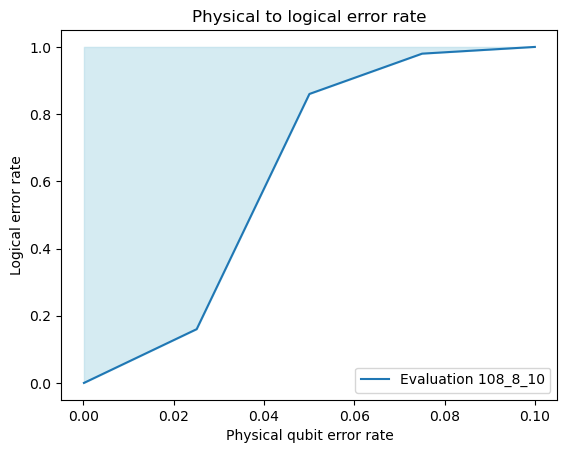
\includegraphics[width=0.95\linewidth]{art/rewardExplained}
    \caption{Physical-to-logical error rate curve explanation. The reward is calculated as the area between the performance curve and the constant function \(1\).}
    \label{fig:reward-explained}
\end{figure}


\subsection{Bivariate Bicycle Codes}
\label{sec:bb}
Bicycle codes are a sub-family of CSS codes, originally defined in~\cite{mackay2004sparse}. Bivariate Bicycle codes were subsequently defined as follows:
\begin{definition}[Bivariate Bicycle code~\cite{bravyi2024high}]
    \label{def:bbcode}
Let \(S_\ell\) be the cyclic shift matrix of size 
\(\ell\times\ell\) and set 
\begin{equation}
X = S_\ell \otimes I_m,\qquad Y = I_\ell \otimes S_m
\end{equation}
And note that \(XY=YX\) and \(X^l=Y^m=I_{lm}\). A BB code is specified by a pair of matrices
\begin{equation}
    A = A_1 + A_2 +A_3, \qquad B=B_1+B_2+B_3
\end{equation}
where each matrix \(A_i\) and \(B_j\) is a power of \(X\) or \(Y\), and subsequent parity check matrices, 
\begin{equation}
    H^X = [A \mid B], \qquad H^Z = [B^\top \mid A^\top].
\end{equation}
\end{definition}
\noindent The definition in~\cite{bravyi2024high} also suggested that the \(A_i\)s should be distinct as to not cancel out (similarly for the \(B_i\)s). 
In this work, we take a slight generalisation of this definition, following~\cite{voss2024multivariate, voss2025multivariate}, by defining polynomials \polynomials{} and subsequently taking:
\begin{equation}
A=a(X) \oplus a(Y)  \qquad B = b(X) \oplus b(Y)     
\end{equation}
\noindent Either definition guarantees the commutation of the resulting stabilizers, since circulant matrices (\(X,Y\) and their powers) commute, as well as a symmetry between the number of \(X\) and \(Z\) stabilizers. The code has length \(n = 2l m\). The code is entirely determined by the coefficients of the four polynomials \polynomials{}. 
This compact parameterisation is important to our RL formulation: 
rather than searching over binary matrices, each of size \((lm) \times (2lm)\), 
the agent searches over a space of four polynomials of degrees at most \(l-1,m-1\) and binary coefficients. 
The reader should be aware that other definitions, narrower and wider, exist in~\cite{panteleev2021degenerate, wang2024coprime, eberhardt2024logical, kovalev2013quantum}.


\subsection{Proximal Policy Optimisation}
\label{sec:ppo}
Loosely speaking, reinforcement learning provides a framework for problems where we make sequential decisions, or ``actions'', 
moving us through ``states'', each associated with a ``reward''.
If we denote the state at time \(t\) by \(s_{t}\) and the action by \(a_{t}\), then a trajectory \(\tau\), 
is a sequence of states and actions, starting at \(t=0\), i.e.:
\begin{equation}
\tau = \{s_i, a_i\}_{i=0}^{\infty}
\end{equation}

\noindent If we further denote the reward by \(r_t(s_{t}, a_{t})\)
then we can look at the discounted cumulative reward:
\begin{equation}
\label{eq:return}
 R(\tau) = \sum_{i=0}^{\infty} \gamma^{k}\cdot r_t 
\end{equation}

\noindent Assuming one starts from a state \(s\), and acting using a policy \(\pi\), we can look at the following two functions: the first is the value function, which tells what is the value of acting using \(\pi\) from state \(s\):
\begin{equation}
    V^{\pi}(s) = \underset{\tau \sim \pi}{E}\left[R(\tau)| s_0 = s\right]
\end{equation}
The second is: if we were to take an action \(a\) (not necessarily using the policy \(\pi\)), what would be the value of continuing the trajectory but sticking to the policy \(\pi\), i.e., the Action-Value function:
\begin{equation}
    Q^{\pi}(s,a) = \underset{\tau \sim \pi}{E} \left[R(\tau)| s_0 = s, a_0 = a\right]
\end{equation}
\noindent The advantage function, is then defined by:
\begin{equation}
A^{\pi}(s,a) = Q^{\pi}(s,a) - V^{\pi}(s)
\end{equation}

\noindent The goal of an RL agent is to learn a parametrized policy, \(\pi_{\theta}\) that maximises the return~\ref{eq:return}.
Policy gradient methods are a family of RL algorithms that learn such policies, and are appealing especially 
when the action and state spaces are either continuous or high-dimensional discrete.
In this work we use Proximal Policy Optimisation (PPO)~\cite{schulman2017proximal}, which forces a policy 
update to stay close to the current policy via a clipped surrogate objective:
\begin{equation}
\begin{split}
    &L^{\text{CLIP}}(\theta) = \\
    &\mathbb{E}_t\!\left[\min\!\left(\rho_t(\theta)\hat{A}_t,\; \text{clip}(\rho_t(\theta), 1-\epsilon, 1+\epsilon)\hat{A}_t\right)\right]
\end{split}
\end{equation}
where \(\rho_t(\theta) = \pi_\theta(a_t|s_t)/\pi_{\theta_{\text{old}}}(a_t|s_t)\) is the importance weight and \(\hat{A}_t\) is an approximation of the advantage function.
In addition to the policy \(\pi_\theta\), PPO also learns an approximation to the value 
function \(V_\phi(s)\). The overall algorithm is summarised in Algorithm~\ref{alg:main}. 
The code we used to apply PPO, once we state the problem in terms of states and actions in Section~\ref{sec:mdp}, 
is almost a drop-in-place reuse of the code explained in~\cite{bou2024torchrl}, and described by Algorithm~\ref{alg:main}.


\subsection{Dataset\label{sec:dataset}}
We accumulated a dataset of BB codes of various parameters as described in Table~\ref{tab:recordCensus}. 
Although it is not strictly needed to carry out PPO training in Algorithm~\ref{alg:main}, 
we used it in supervised learning manner, in an effort to start PPO from a better-than-random policy weights. 
We discuss this strategy, as well as our findings in Section~\ref{sec:critic}.
The collection was done by setting the agent to high exploration mode (by enforcing high entropy) and setting the environment to log them.
\begin{figure}[htbp]
    \centering
    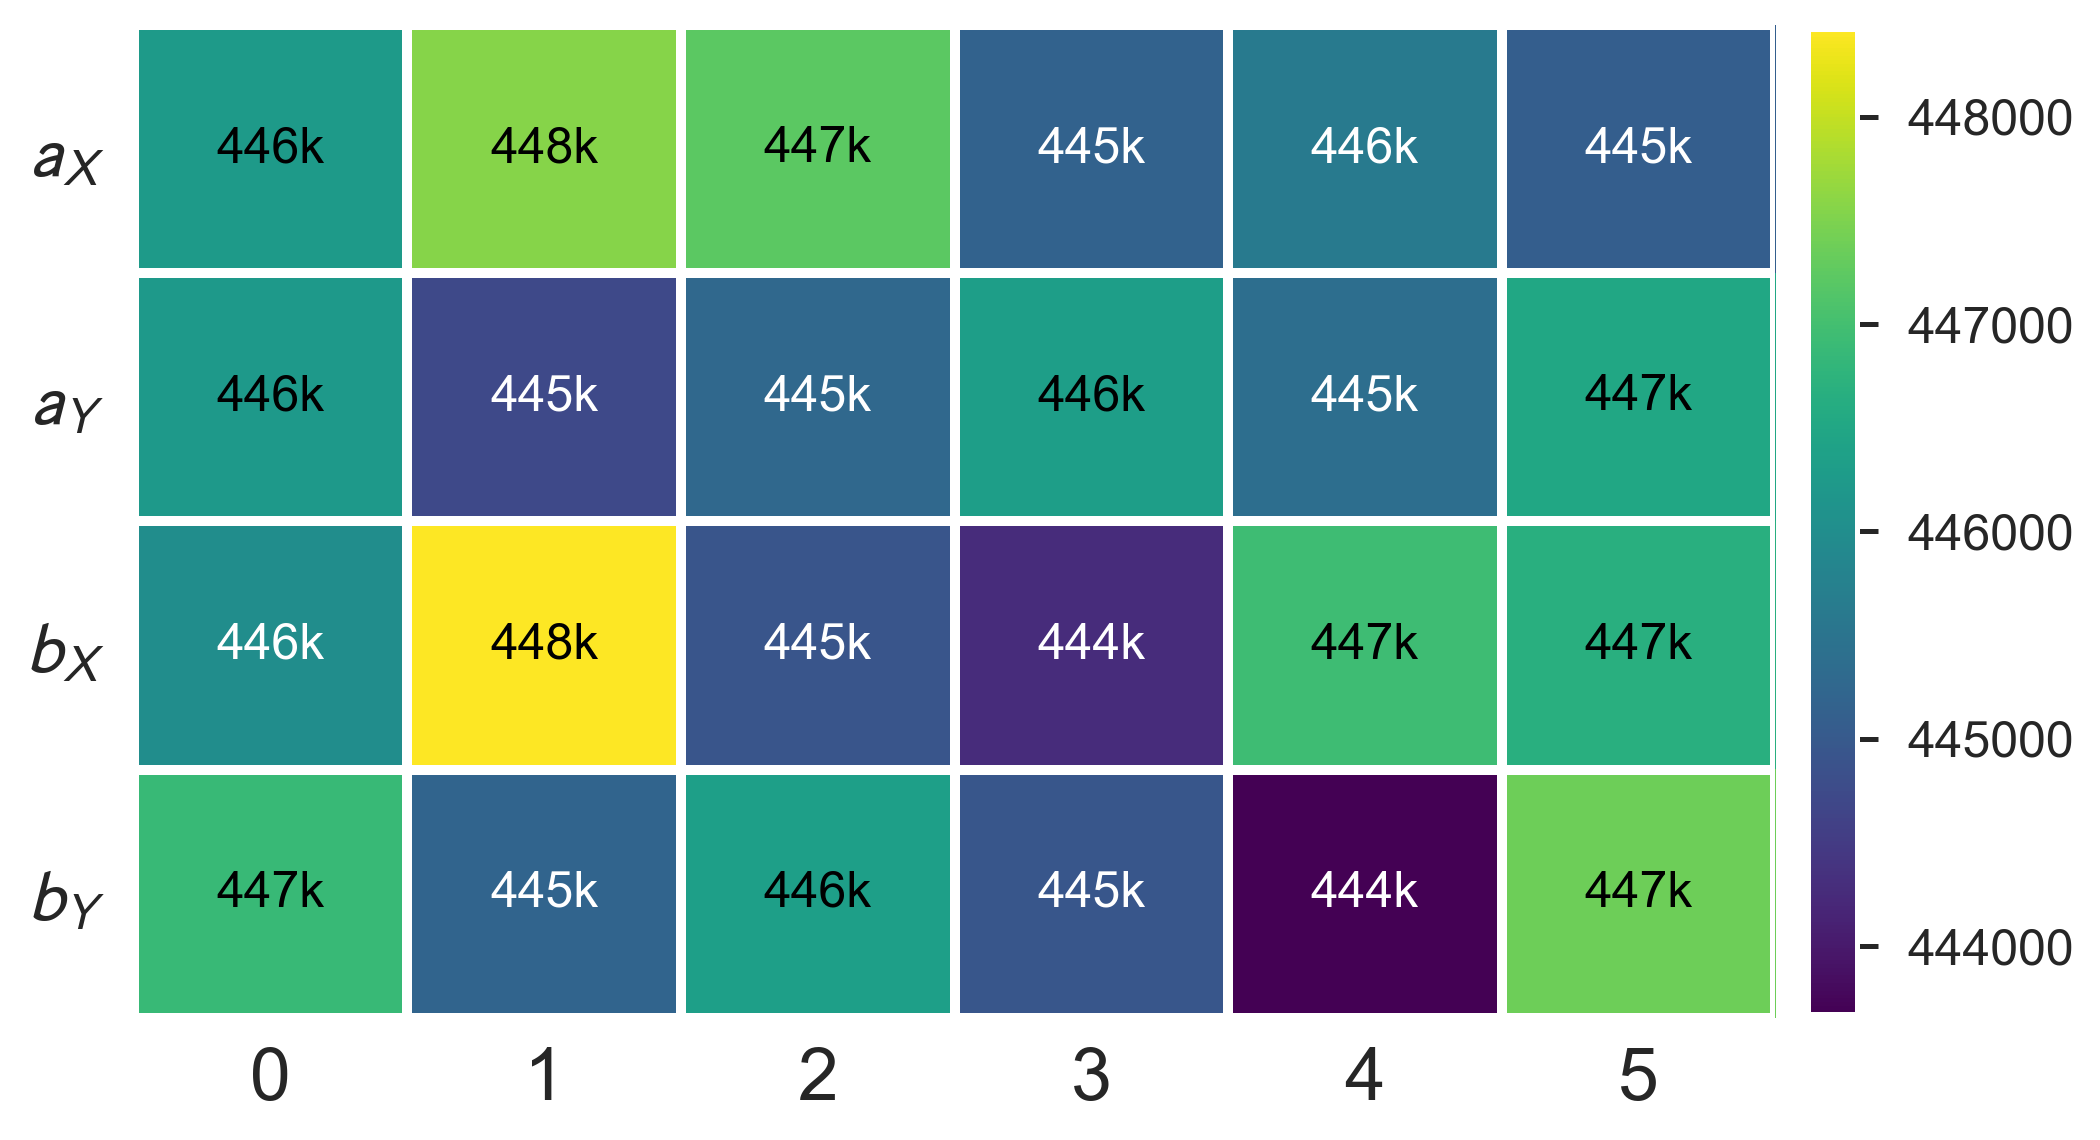
\includegraphics[width=0.9\linewidth]{./art/dataset/coefficientUsage_l_6_m_6_error_range_union.png}
     \label{fig:coefficientsHeatmap-6-6}
     \caption{Coefficient heatmap showing hits per coefficient index for the codes in the \(l=6, m=6\) dataset. Similar figures for other code sizes are provided in~\ref{appendix:dataset}, Figure~\ref{fig:coefficientsHeatmap-rest}.}
\end{figure}
A more extensive statistical analysis of this dataset can be found in Appendix~\ref{appendix:dataset}. 
The dataset itself, as well as the code used to produce the figures describing is available for public use~\cite{sella2026bbcodesdataset}.
The dataset provides ``labels'', i.e., the monte-carlo evaluation of each code over \(50\) samples per point. 
A typical .jsonl file in the repository contains multiple code records, each with the code parameters 
(\(l,m\), \polynomials{}, number of logical qubits) 
as well as the error range over which the code was evaluated, and the corresponding logical error counts. 
We note that the codes were not evaluated until a fixed number\footnote{The usual methodology is to observe \(100\) errors for high confidence.} 
of errors were observed, but rather over a fixed number of samples, as we use in training.

\begin{figure}[htbp]
    \centering    
    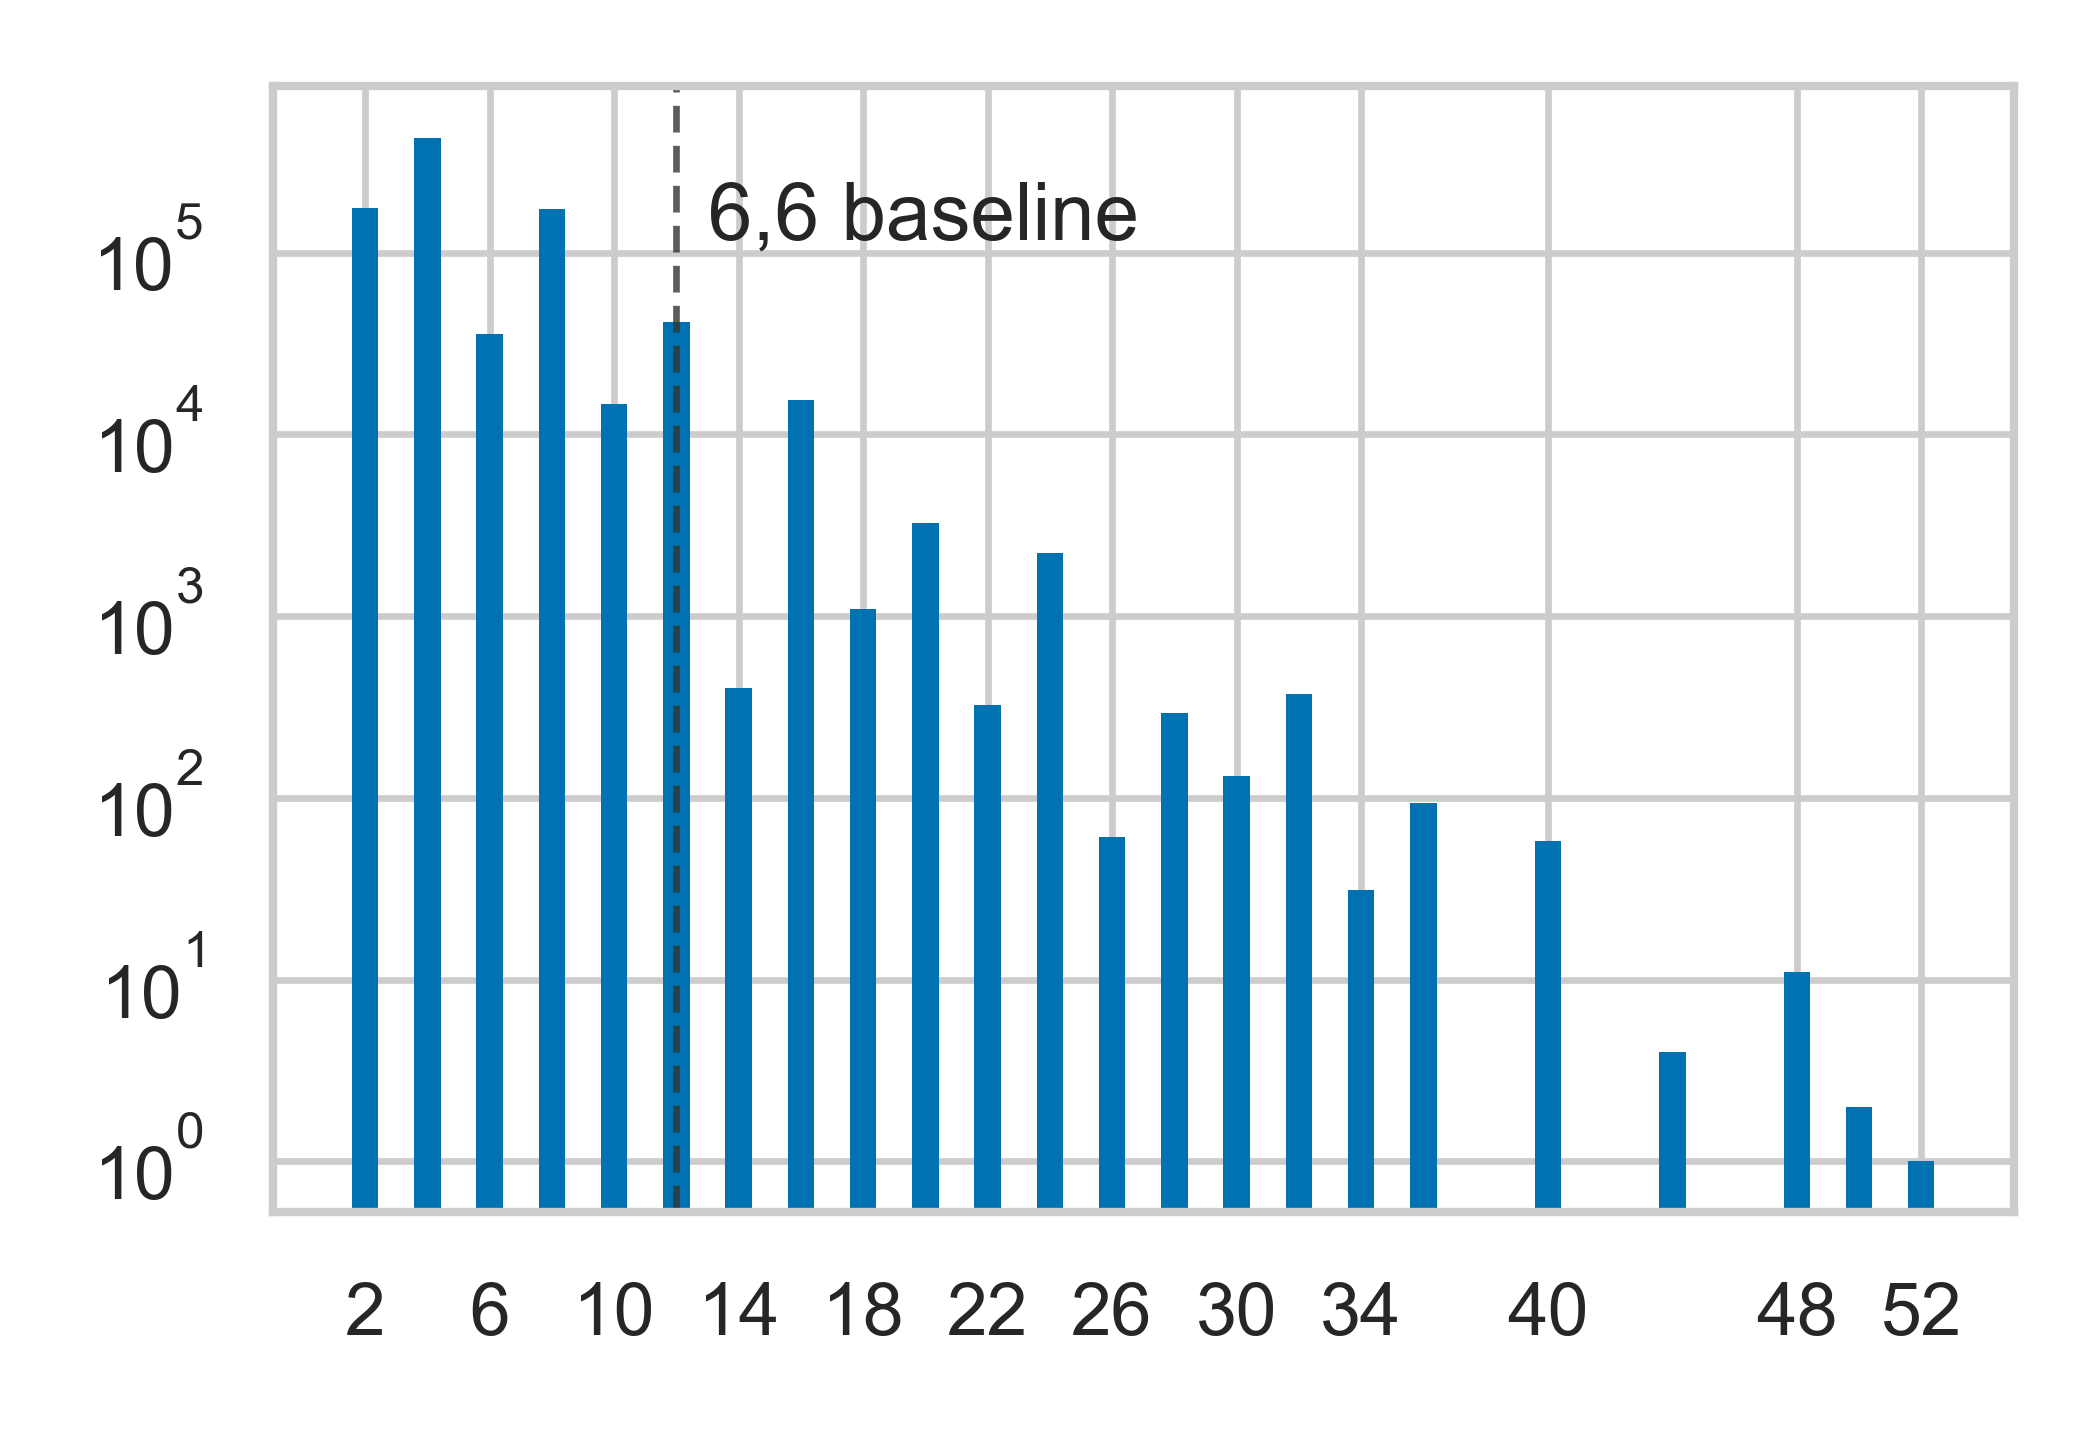
\includegraphics[width=0.9\linewidth]{./art/dataset/kDistribution_l_6_m_6.png}
  \caption{Distribution of the number of logical qubits for the codes in the \(l=6, m=6\) dataset. Similar figures for other code sizes are provided in~\ref{appendix:dataset}, Figure~\ref{fig:kDistribution-rest}}
  \label{fig:kDistribution-6-6}
\end{figure}

\noindent It should be stated that, the representation of a BB code using the polynomials \polynomials{} is not unique, 
and the dataset contains duplicates. Two evaluations of the same code by the same decoder are independent Bernoulli trials of the same probability, so pooling them could improve the estimate.


